% Figure from MATH 591 notes, section 4. Compile with the notes preamble.
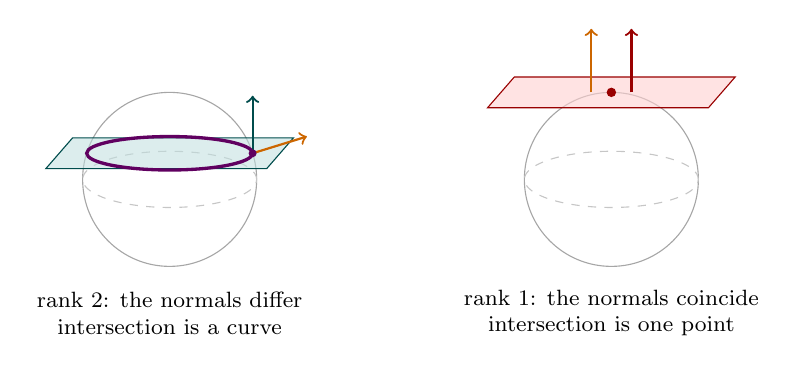
\begin{tikzpicture}[scale=0.85]
\draw[gray!70] (0,0) circle (1.3);
\draw[gray!45,dashed] (0,0) ellipse (1.3 and 0.42);
\fill[teal!25,opacity=0.55] (-1.85,0.16) -- (1.45,0.16) -- (1.85,0.62) -- (-1.45,0.62) -- cycle;
\draw[teal!60!black] (-1.85,0.16) -- (1.45,0.16) -- (1.85,0.62) -- (-1.45,0.62) -- cycle;
\draw[violet!75!black,very thick] (0,0.39) ellipse (1.24 and 0.25);
\draw[orange!80!black,->,thick] (1.24,0.39) -- (2.05,0.64);
\draw[teal!60!black,->,thick] (1.24,0.39) -- (1.24,1.25);
\fill[violet!75!black] (1.24,0.39) circle (1.7pt);
\node[font=\footnotesize,align=center] at (0,-2.0) {rank $2$: the normals differ\\ intersection is a curve};
\begin{scope}[xshift=6.6cm]
\draw[gray!70] (0,0) circle (1.3);
\draw[gray!45,dashed] (0,0) ellipse (1.3 and 0.42);
\fill[red!18,opacity=0.6] (-1.85,1.07) -- (1.45,1.07) -- (1.85,1.53) -- (-1.45,1.53) -- cycle;
\draw[red!60!black] (-1.85,1.07) -- (1.45,1.07) -- (1.85,1.53) -- (-1.45,1.53) -- cycle;
\draw[orange!80!black,->,thick] (-0.3,1.3) -- (-0.3,2.25);
\draw[red!60!black,->,thick] (0.3,1.3) -- (0.3,2.25);
\fill[red!60!black] (0,1.3) circle (2pt);
\node[font=\footnotesize,align=center] at (0,-2.0) {rank $1$: the normals coincide\\ intersection is one point};
\end{scope}
\end{tikzpicture}
